\documentclass[a4paper,10pt]{article}
\usepackage[right=1in,left=1in,top=0.7in,bottom=0.7in]{geometry}
\usepackage{lipsum}
\usepackage{graphicx}
\usepackage{float}
\usepackage{cite}
\usepackage{color}
\usepackage{caption}

% \usepackage{listings}
% \usepackage{hyperref}
% \usepackage{textgreek}

\renewcommand{\familydefault}{\sfdefault}
% \setmainfont{Neue Montreal}

\begin{document}
    \begin{titlepage}
        \begin{center}
            
\includegraphics[height=7.5em]{../resources/unilogo.png}
            
            \vspace{10em}
            {\LARGE Laboratory Protocol} \\ 
            {\huge\bfseries Characterization of Protein Stability,\\ Catalysis and Aggregation}
            
            \vspace{5em}
            {\large\bfseries Molecular Biology and Biochemistry of Life}\\
            {\large Winter Semester 2023-24}
            
            \vspace{12em}
            {\bfseries Authors} \\ 
            Masine Janet Tränkner\\
            Syed Alisamar Husain
            
            \vspace{5em}
            {\bfseries Supervisor} \\ Dr.\ Titus M. Franzmann
        \end{center}
    \end{titlepage}
    \pagebreak

    \tableofcontents
    \listoffigures
    \vspace{3em}
    {\noindent\Large\bfseries Author Information \vspace{0.75em}}\\
    \noindent\large Masine Janet Tränkner\\
    {\small MSc. Computational Modelling and Simulation}\\
    {\small Matriculation Number --- 5186813}\\
    {\it\small masine\_janet.traenkner@mailbox.tu-dresden.de}\\\vspace{0.5em}
    
    \noindent\large Syed Alisamar Husain\\
    {\small MSc. Computational Modelling and Simulation}\\
    {\small Matriculation Number --- 5198172}\\
    {\it\small syed\_alisamar.husain@mailbox.tu-dresden.de}
    \pagebreak

    \section{Temperature Induced Unfolding Transitions}
        The goal in this experiment is to determine the stability of the proteins Lysozyme and BSA 
        (Bovine Serum Albumin) at different concentrations, 2.5, 5 and 10 $\mu M$, by inducing unfolding 
        transitions through temperature changes.
        We detect unfolding using Fluorescence spectroscopy by measuring emission at 
        two wavelengths, 330nm and 350nm, and we expect to see a sharp increase in the ratio
        of these emissions when the protein unfolds.

        \subsection*{Measurements}
            The temperature was increased from 25 °C to 95 °C, at a rate of 2 °C per minute,
            and corresponding fluorescence at wavelengths 350nm and 330nm was measured and 
            is plotted in Figure~\ref{fig:lys_flr} (a) and (b) for Lysozyme, and in 
            Figure~\ref{fig:bsa_flr} (a) and (b) for BSA, respectively.

            \begin{itemize}
                \item {\bfseries Lysozyme --- Fluorescence vs. Temperature}
                \begin{figure}[H]
                    \centering
                    \begin{tabular}{cc}
                        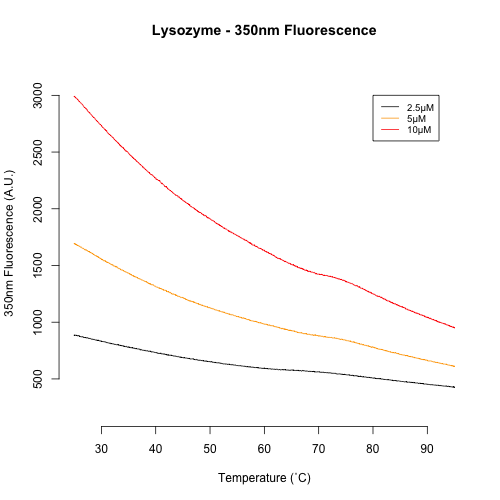
\includegraphics[width=200px]{../resources/unfolding_lys_350.png} &
                        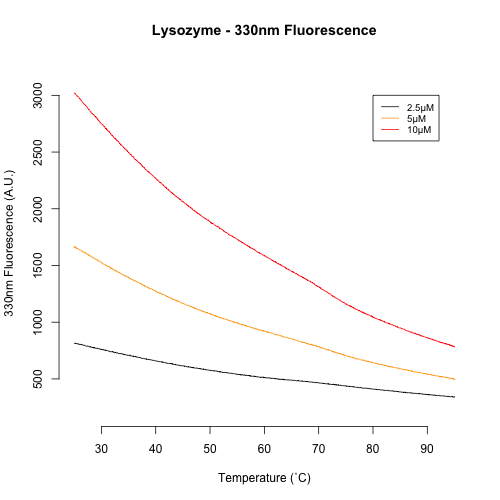
\includegraphics[width=200px]{../resources/unfolding_lys_330.png} \\
                        (a) & (b)\\
                    \end{tabular}
                    \caption{\it Lysozyme Fluorescence at wavelengths (a) 350nm and (b) 330nm}\label{fig:lys_flr}
                \end{figure}
                
                \item {\bfseries Bovine Serum Albumin (BSA) --- Fluorescence vs. Temperature}
                \begin{figure}[H]
                    \centering
                    \begin{tabular}{cc}
                        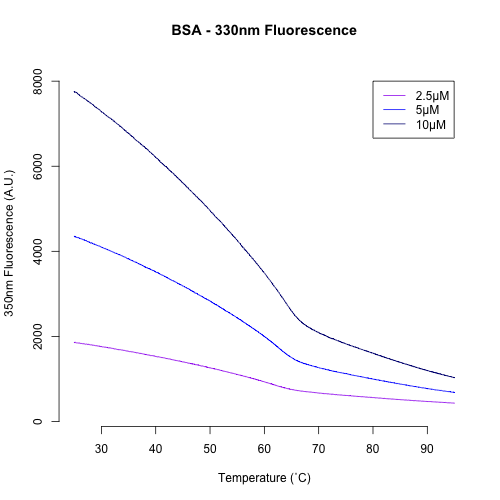
\includegraphics[width=200px]{../resources/unfolding_BSA_350.png} &
                        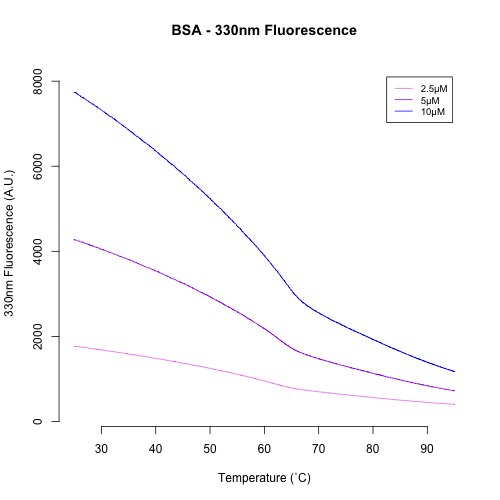
\includegraphics[width=200px]{../resources/unfolding_BSA_330.png} \\
                        (a) & (b)\\
                    \end{tabular}
                    \caption{\it BSA Fluorescence at wavelengths (a) 350nm and (b) 330nm}\label{fig:bsa_flr}
                \end{figure}
            \end{itemize}

        \subsection*{Analysis}
            The Fluorescence Ratio graph (Fig.~\ref{fig:temp_ratio}(a) and Fig.~\ref{fig:temp_ratio}(b)) was used to 
            approximate the transition midpoint. 
            Stability in the folded state arises from various interactions within the polypeptide. 
            However, upon surpassing a threshold temperature, the polypeptide 
            transitions to an unstable state. Consequently, as temperature increases, the population 
            of unfolded molecules also rises. This process behaves differently for the two proteins. 

            For Lysozyme, a low ratio can be observed at the beginning, which indicates that 
            the folded state predominates. With increasing temperature, this confirmation changes 
            up to a threshold temperature and the transition of the molecules into the unfolded state, 
            and accordingly the ratio also increases.
            \begin{figure}[H]
                \centering
                \begin{tabular}{cc}
                    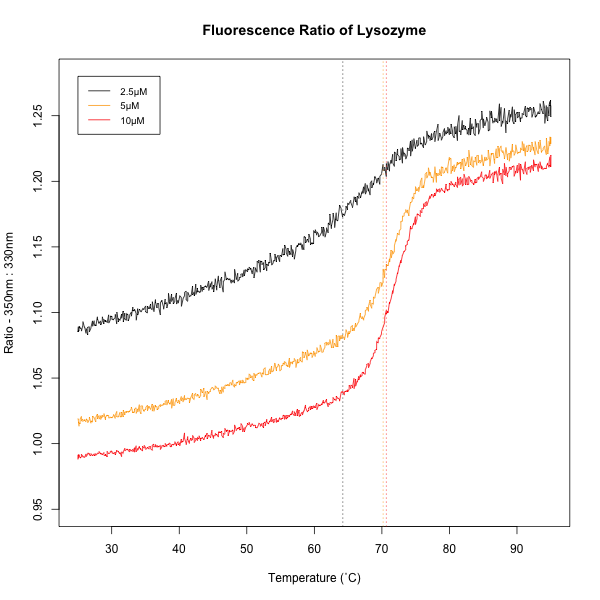
\includegraphics[width=215px]{../resources/unfolding_lys_ratio.png} &
                    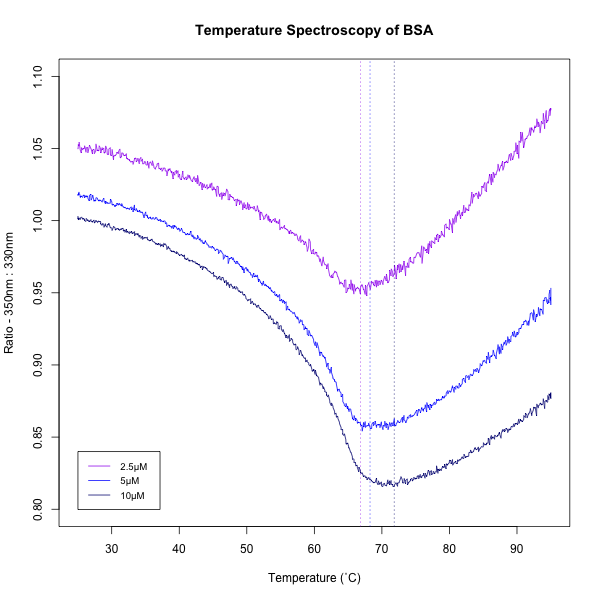
\includegraphics[width=215px]{../resources/unfolding_BSA_ratio.png} \\
                    (a) & (b)\\
                \end{tabular}
                \caption{\it Ratio of Fluorescence at 350nm to 330nm for (a) Lysozyme and (b) BSA}
                \label{fig:temp_ratio}
            \end{figure}
            
            The opposite can be observed for BSA. Here, the ratio is already high at the start of 
            the process and falls down to a certain threshold temperature. From this point, the ratio 
            increases for all concentrations and thus also the amount of proteins in the unfolded state.
            
            \begin{minipage}{0.49\textwidth}
                \begin{figure}[H]
                    \centering
                    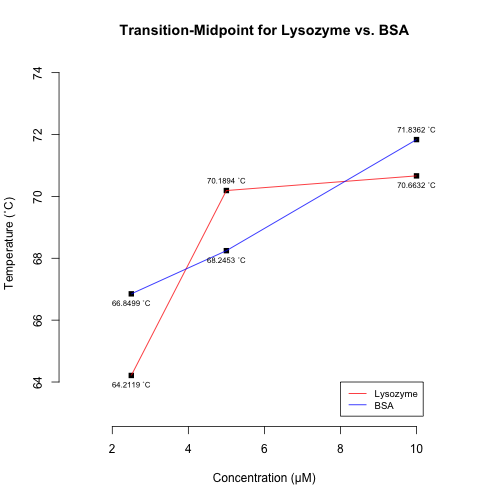
\includegraphics[width=\textwidth]{../resources/unfolding_tempVconc.png}
                    \caption{\it Transition midpoints relative to\\concentration for Lysozyme and BSA}
                    \label{fig:temp_v_mid}
                \end{figure}
            \end{minipage}
            \begin{minipage}{0.49\textwidth}
                \vspace{-2em}
                The transition midpoints relative to concentration are plotted in Figure~\ref{fig:temp_v_mid}.
                The overall stability of the folded proteins increases with protein concentration.\\

                \begin{tabular}{| c | c | c | c |}
                    \hline
                    Sample & 2.5 $\mu M$ & 5 $\mu M$ & 10 $\mu M$ \\
                    \hline
                    \hline
                    Lysozyme & 64.21 $^{\circ}$C & 70.19 $^{\circ}$C & 70.66 $^{\circ}$C \\
                    BSA & 66.85 $^{\circ}$C & 68.24 $^{\circ}$C & 71.83 $^{\circ}$C \\
                    \hline
                \end{tabular}
                \begin{center}
                    \small Table 1: \it Transition Midpoints vs. Concentration
                    \label{tab:midpoints}
                \end{center}

                The limit temperature for BSA appears to increase linearly with the concentration. 
                The limit temperature for Lysozyme increases drastically initially until 5$\mu M$.\\
                After this point, the midpoint appears to increase only slightly with concentration.
            \end{minipage}
    \pagebreak
    
    \section{Lysozyme Aggregation Assay}
        In this experiment, aggregation of Lysozyme was studied to understand protein aggregation, 
        where unfolded polypeptide chains of the proteins Lysozyme and Hsp26 associate irreversibly, 
        leading to the formation of large particles that scatter light.
        
        \subsection*{Measurements}
            Detecting the actual scattering of light is a challenging task that requires more equipment.
            Instead, we measure absorbance as a proxy for scattering using a pulsed spectrometer.
            We choose a wavelength which we know is not absorbed by anything in the mixture and 
            we use that fact to say all of the intensity reduction is because of scattered light.
            As protein aggregation increases, more light is scattered by the sample. 
            \begin{figure}[H]
                \centering
                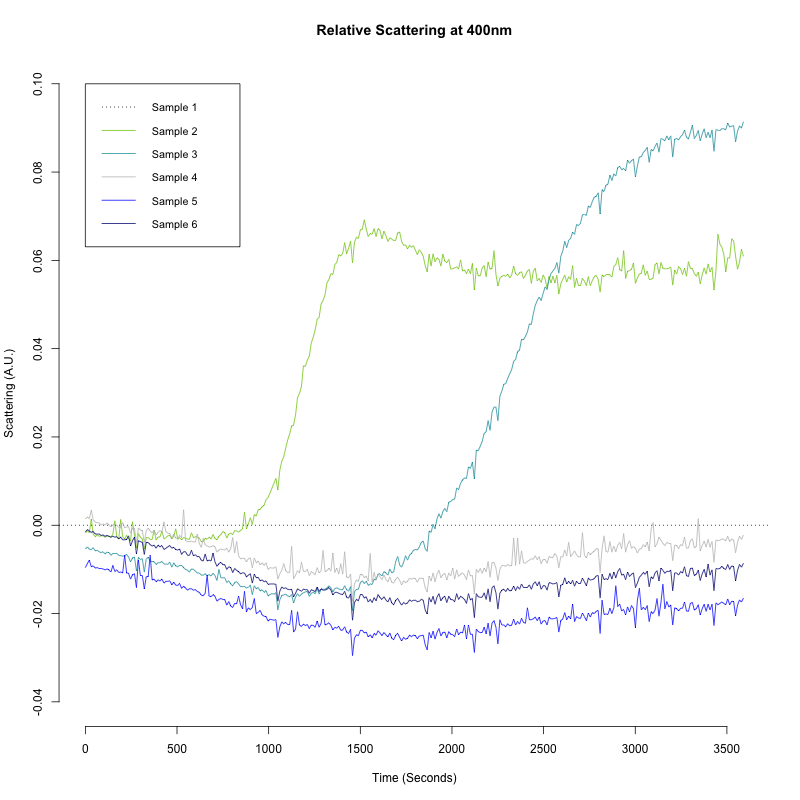
\includegraphics[width=350px]{../resources/aggregation_main.png}
                \caption{\it Scattering recorded as a function of time.}\label{fig:agg_main}
            \end{figure}

        \subsection*{Analysis}
            At low concentrations of Hsp26 (samples 2 and 3 in Figure~\ref{fig:agg_main}), 
            Lysozyme aggregation is not effectively inhibited. 
            Thus the presence of TCEP in the solution increases scattering. 
            But it can also be seen that a higher concentration of Hsp26 in sample 3 delays the aggregation.
            
            However, when the concentration of Hsp26 matches that of Lysozyme in sample 4, 
            aggregation is prevented resulting in lower absorbance.
            The control samples 5 and 6 lacking Lysozyme and denaturant exhibit no absorbance change at 400nm. 
            Only Samples 2 and 3 allow for the determination of an apparent halftime, which are $T^{S2}_{50\%} = 1200.30s$
            and $T^{S3}_{50\%} = 2422.34s$ respectively, as their curves display a change of conformation.
            Doubling the concentration appears to double the halftime, but this is not conclusive from just two samples.
    \pagebreak
    
    \section{Michaelis-Menten Kinetics}
        Lactatdehydrogenase (LDH) catalyzes the reaction conversion of Pyruvate into Lactate. 
        In order to measure its activity the fluorescence of NADH, the cofactor of LDH, is measured 
        under 340nm light. As NADH is converted to NAD$^+$, this fluorescence reduces and reaches a 
        steady state when the reaction reaches equilibrium. We measure how fast this happens to determine
        the rate of reaction and find the Michaelis-Menten constants.
        
        \subsection*{Measurements}
            We measure the absorbance of 340nm light through a sample of the reaction mixture over time
            and plot this in Figure \ref{fig:mm_rates}. The slopes of these lines are directly proportional
            to the rates of reaction for each sample.
            \begin{figure}[H]
                \centering
                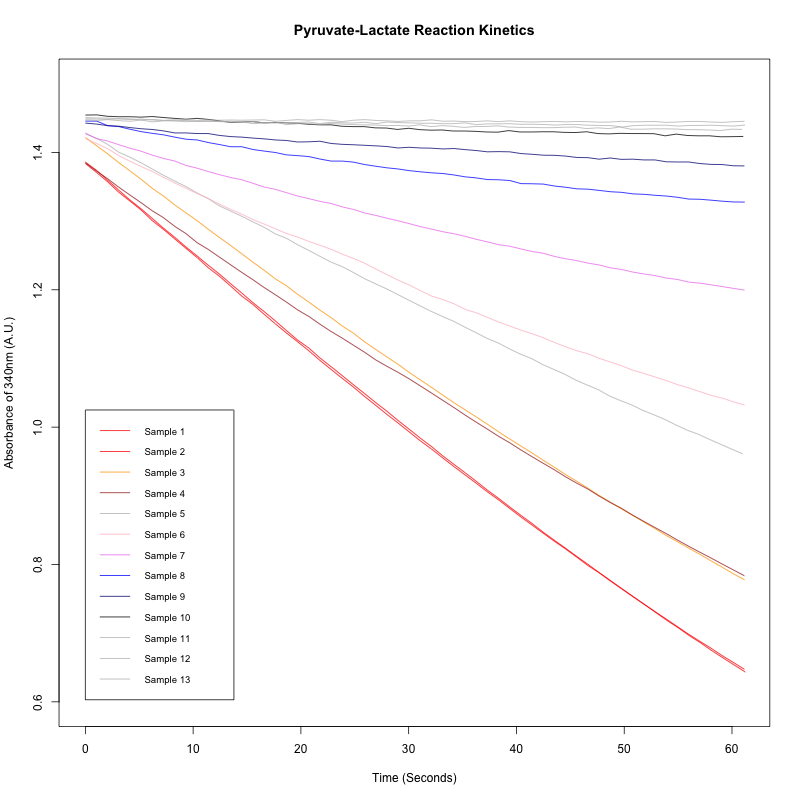
\includegraphics[width=350px]{../resources/kinetics_rates.png}
                \caption{\it Absorbance  as a function of time for different concentrations of Pyruvate}\label{fig:mm_rates}
            \end{figure}
            
            \subsection*{Analysis}
                The Michaelis-Menten plot (Fig.~\ref{fig:mm_plot}(a)) and the Lineweaver-Burk plot 
                (Fig.~\ref{fig:mm_plot}(b)) can be plotted from reaction rates derived 
                from change of absorbance over time, relative to the concentration of substrate. 
                It is evident that for low substrate concentrations, the rate of the reaction increases 
                linearly with increasing substrate concentration. As the substrate concentration increases, 
                the rate of the reaction eventually reaches a maximum value ($v_{max}$). 
                In this region, the active sites of the enzyme are largely occupied by the substrate, 
                and the rate becomes independent of further increases in substrate concentration.

                To find the maximum rate of reaction ($v_{max}$) and the Michaelis-Menten constant ($K_m$),
                we fit a linear model to the data, and the model estimates will give us an approximation of these constants.

                The Michaelis-Menten equation
                $ \frac{1}{V} = \frac{K_m}{v_{max}}\frac{1}{[S]} + \frac{1}{v_{max}} $
                is of the form
                $ y = \beta_1x + \beta_0 $.

                \begin{center}
                    Thus we have,
                    $ v_{max} = \frac{1}{\beta_0} $ and $ K_m = \frac{\beta_1}{\beta_0}  $
                \end{center}

                \begin{figure}[H]
                    \centering
                    \begin{tabular}{cc}
                        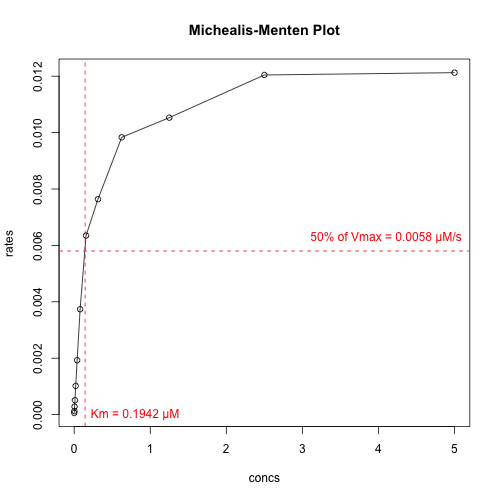
\includegraphics[width=220px]{../resources/kinetics_mmplot.png} &
                        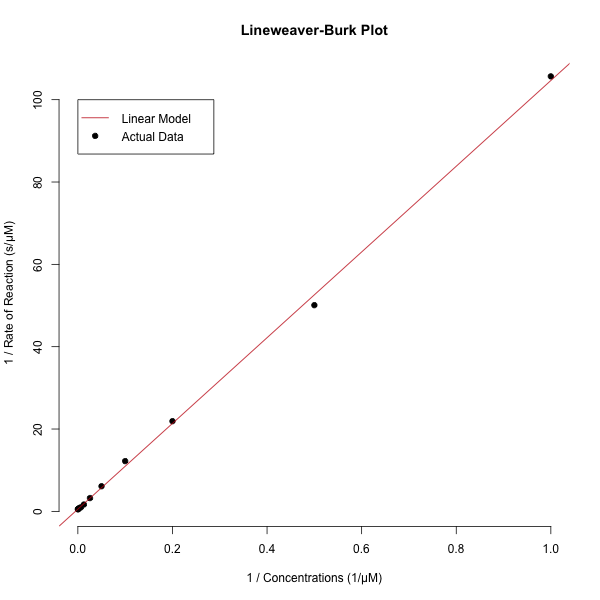
\includegraphics[width=220px]{../resources/kinetics_lbplot.png} \\
                        (a) & (b)\\
                    \end{tabular}
                    \caption{\it Michaelis-Menten plot and Lineweaver-Burk plot}\label{fig:mm_plot}
                \end{figure}

                \noindent From the linear model estimates we get $v_{max}$ = 1.8649 $\mu M$/s and for $K_m$ = 194.19 $\mu M$.\\
                We mark the value $v_{max}/2$ on the Michaelis-Menten plot (Fig.~\ref{fig:mm_plot}(a)), which can
                also give us the value of $K_m$ graphically. 
                In the Lineweaver-Burk plot (Fig.~\ref{fig:mm_plot}(b)) the slope of the fitted line indicates 
                the ratio $\frac{K_m}{v_{max}}$.\\

                To find the change in NADH concentration for each sample, we can use the absorbance formula
                of Lambert-Beer, $A = \epsilon d C$, we have,
                \begin{center}
                    $\Delta A = \epsilon d \Delta C$
                \end{center}

                \begin{center}
                    Thus, $\Delta C = \frac{\Delta A}{\epsilon d}$,
                    where $\epsilon = 6220 M^{-1} cm^{-1}$ and $d = 1$ cm.
                \end{center}
                
                \noindent Change in NADH concentration is calculated from the change in absorbance.\\
                \begin{center}
                    \begin{tabular}{ c | c | c }
                        [Pyruvate] ($\mu M$) & $\Delta$A (A.U.) & $\Delta$[NADH] ($\mu M$) \\
                        \hline 
                        \hline 
                        5000 & 0.7425 & 119.3729 \\
                        2500 & 0.7365 & 118.4083 \\
                        1250 & 0.6441 & 103.5530 \\
                         625 & 0.6013 & 96.67202 \\
                         313 & 0.4660 & 74.91961 \\
                         156 & 0.3884 & 62.44372 \\
                          78 & 0.2286 & 36.75241 \\
                          39 & 0.1179 & 18.95498 \\
                          20 & 0.0623 & 10.01607 \\
                          10 & 0.0311 & 4.999999 \\
                           5 & 0.0173 & 2.781350 \\
                           2 & 0.0076 & 1.221864 \\
                           1 & 0.0036 & 0.578778 \\
                    \end{tabular}
                \end{center}

    \pagebreak

    \section{UV/VIS Spectroscopy of NADH}
    The NADH (Nicotinamide adenine dinucleotide reduced) UV-Visible spectrum has two absorption maxima at 
    208nm, 260 nm and 340 nm. We measure the absorbance UV/VIS spectroscopy at different concentrations and thus 
    try to determine the concentration of the original stock of NADH using the Lambert-Beer law.
    It is expected that the absorbance increases with increasing NADH concentration. 
    
        \subsection*{Measurements}
            \begin{figure}[H]
                \centering
                \begin{tabular}{c c}
                    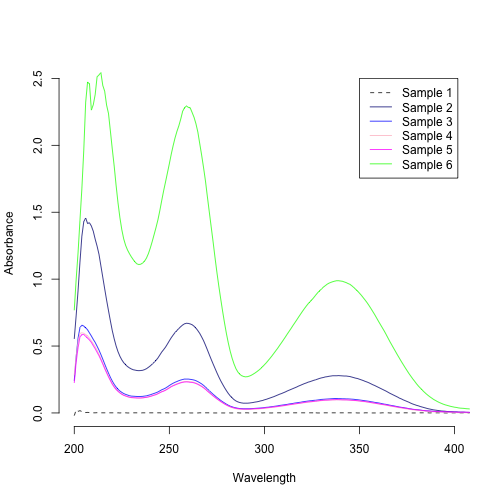
\includegraphics[width=215px]{../resources/absorption_r1_spectrum.png} &
                    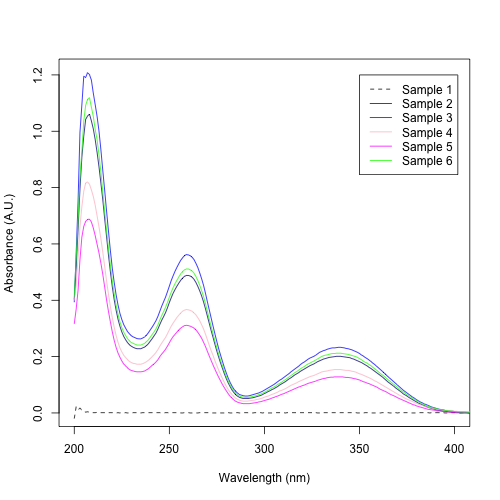
\includegraphics[width=215px]{../resources/absorption_r2_spectrum.png} \\
                    (Attempt 1) & (Attempt 2)\\
                \end{tabular}
                \caption{\it Absorbance spectrum of NADH for different concentrations}\label{fig:abs_spectrum}
            \end{figure}

        \subsection*{Analysis}
            \begin{minipage}{0.49\textwidth}
                \vspace{-2em}
                We expected to see an increase in the absorbance with increase in concentrations and 
                to see a straight line in the plot between samples of unknown concentrations and absorbance.
                
                However, according to Figure~\ref{fig:abs_340}, the absorbance increases from sample 1 to 3, 
                then increases for the samples 4 and 5 and again increases for sample 6, 
                without exceeding the highest absorbance of sample 2. 

                The experiment was repeated with different equipment, different pipette and different
                person preparing the samples, to eliminate causes of error. But the data obtained 
                was still not as expected.
            \end{minipage}
            \hspace{0.01\textwidth}
            \begin{minipage}{0.49\textwidth}
                \begin{figure}[H]
                    \centering
                    \caption{\it Absorbance at 340nm vs. concentration}\label{fig:abs_340}
                    
\includegraphics[width=0.98\textwidth]{../resources/absorption_340.png}
                \end{figure}
            \end{minipage}\\

            Our best reasoning for the cause of this discrepancy is that while washing the cuvette
            used in the spectrometer between samples, there were droplets of water left in the 
            slot which caused dilution of the sample.
            Another possibility is that due to the time taken to prepare samples, the ambient 
            temperature caused degradation of NADH.

            We have tried to rectify this situation by using the points that are increasing with
            concentration as expected to fit a linear regression model and predict those absorbance
            values that should have been observed for these concentrations.

            \begin{minipage}{0.49\textwidth}
                \begin{figure}[H]
                    \centering
                    \caption{\it Predicted Absorbance at 340nm}\label{fig:abs_340_pred}
                    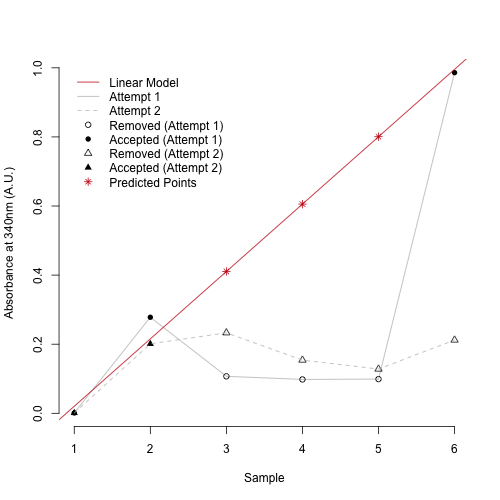
\includegraphics[width=\textwidth]{../resources/absorption_340_pred.png}
                \end{figure}
            \end{minipage}
            \hspace{0.01\textwidth}
            \begin{minipage}{0.49\textwidth}
                \vspace{-7em}
                The accepted and predicted values of\\ absorbance are listed in this table.\\
                The predicted values are written in {\it italics}.\\
                
                \begin{tabular}{| c | c | c |}
                    \hline 
                    {\bfseries Sample} & {\bfseries Abs (A.U.)} & {\bfseries Source} \\
                    \hline 
                    \hline 
                    1 & 0.001 & Run 2 \\
                    2 & 0.201 & Run 2 \\
                    3 & {\it 0.410} & * \\
                    4 & {\it 0.605} & * \\
                    5 & {\it 0.801} & * \\
                    6 & 0.986 & Run 1 \\
                    \hline
                \end{tabular}
            \end{minipage}\\

            Now by using the Lambert-Beer law $A = \epsilon d C$ and using the formula
            $C_1 V_1 = C_2 V_2$, we can find the initial stock concentration of NADH.
            \begin{center}
                $ C = \frac{A}{\epsilon d} \mu M$ and $ C_2 = \frac{C_1 V_1}{V_2} $
                \vspace{0.5em}
                
                Thus $ C_2 = \frac{A V_1}{\epsilon d V_2}$ where,\\
                \vspace{0.5em}

                \begin{tabular}{c c}
                    $ V_2 = [0,1,2,3,4,5] \mu L $ & $ V_1 = 1000 \mu L $, \\
                    $\epsilon = 6220 M^{-1} cm^{-1}$ & $d = 1$ cm.\\
                \end{tabular}
            \end{center}

            Using this formation for all the samples we get mean stock concentration of 
            {\bfseries 32.328 mM}.
    \pagebreak

\end{document}